%% Knowledge-Based Systems -- Short Communication (Elsevier elsarticle, numbered references)
%% Compile: pdflatex main && bibtex main && pdflatex main && pdflatex main (or tectonic main.tex)
\documentclass[preprint,12pt]{elsarticle}
\biboptions{sort&compress}
\usepackage{amssymb,amsmath}
\usepackage{graphicx}
\usepackage{booktabs}
\usepackage{makecell}
\usepackage{array}
\usepackage{tabularx}
\usepackage[hidelinks]{hyperref}
\usepackage{xurl}
\journal{Knowledge-Based Systems}
%% Single-line first-page footer (avoids a 2.6pt overfull box from the class default)
\makeatletter
\def\ps@pprintTitle{\let\@oddhead\@empty\let\@evenhead\@empty
\def\@oddfoot{\footnotesize\itshape Preprint submitted to \@journal\hfill\today}%
\let\@evenfoot\@oddfoot}
\makeatother
%% Table 1 symbols: full / partial / absent
\newcommand{\yes}{$\checkmark$}
\newcommand{\prt}{($\checkmark$)}
\newcommand{\no}{$\times$}
\newcolumntype{L}[1]{>{\raggedright\arraybackslash}p{#1}}
\newcolumntype{C}[1]{>{\centering\arraybackslash}p{#1}}

\begin{document}
\begin{frontmatter}

\title{Fuzzy--Neural Decision Intelligence for Cost-Aware Cyber Alert Triage\tnoteref{t1}}
\tnotetext[t1]{Article type: Short Communication.}

\author[mu]{Sai Nithin Erigineni\corref{cor1}}
\ead{serigineni@midwest.edu}
\cortext[cor1]{Corresponding author.}
\address[mu]{DBA, Midwest University, 851 Parr Rd, Wentzville, MO 63385, United States}

\begin{abstract}
Security operations centres (SOCs) usually turn detector scores into actions with a single hand-set threshold. We treat alert triage as a knowledge-based decision problem: a multilayer perceptron (MLP) estimates attack propensity, fuzzy membership functions map it to Low, Medium and High risk bands, and three production rules assign Monitor, Soft-block or Escalate. On 20,000 NSL-KDD test alerts, gradient boosting is the stronger detector (ROC-AUC 0.947 against 0.908), yet on the same MLP scores the rule base lowers the mean triage cost to 3.068 (95\% CI [3.016, 3.118]), against 3.264 for a 0.5 threshold and 4.309 for top-20\% escalation (both Wilcoxon $p<10^{-100}$), and raises attack coverage from 0.655 to 0.686. It is cheaper than both crisp rules in all ten repeated runs ($p=0.002$) and than the threshold at every tested missed-attack cost. The gain comes from the Soft-block band, and a Bayes cost rule is cheaper still (2.164).
\end{abstract}

\begin{keyword}
Fuzzy logic \sep Neural networks \sep Decision intelligence \sep Intrusion detection \sep Alert triage \sep Cost-sensitive decisions \sep Knowledge-based systems
\end{keyword}
\end{frontmatter}
\enlargethispage{\baselineskip}

%% ---------------------------------------------------------------------------
\section{Introduction}
\label{sec:intro}
Security operations centres (SOCs) collect, analyse and respond to security alerts~\cite{vielberth2020}, but intrusion detectors produce far more alerts than analysts can investigate, most of them false positives~\cite{albasheer2022}. Intrusion-detection research, from fuzzy and neuro-fuzzy detectors~\cite{toosi2007,hamamoto2018} to deep networks trained on NSL-KDD~\cite{vinayakumar2019,su2020}, usually ends with a risk score judged by accuracy or by the area under the receiver operating characteristic curve (ROC-AUC). A SOC manager instead has to decide which alerts to monitor, contain or escalate under limited analyst capacity and unequal error costs. Three-way decisions choose among acceptance, rejection and deferment under stated losses~\cite{yao2010}, and SOC studies learn when to defer alerts to analysts~\cite{jalalvand2027} or rank them by reinforcement learning~\cite{wang2024alertpro}, but these designs do not assign graded actions through readable rules.

\begin{table}[!t]
\centering
\caption{Related work compared by design property, because data sets and tasks differ.}
\label{tab:rw}
{\scriptsize\setlength{\tabcolsep}{2.5pt}
\begin{tabularx}{\linewidth}{@{}l>{\raggedright\arraybackslash}Xlcccc@{}}
\toprule
Study & Approach & Data & Cost & Rules & Graded & Tests \\
\midrule
Toosi~\cite{toosi2007} & Neuro-fuzzy + genetic tuning & KDD Cup 99 & \prt & \yes & \no & \no \\
Hamamoto~\cite{hamamoto2018} & Genetic signature + fuzzy logic & Campus IP flows & \no & \yes & \no & n.r. \\
Vinayakumar~\cite{vinayakumar2019} & Deep neural network & NSL-KDD + 5 others & \no & \no & \no & \no \\
Gupta~\cite{gupta2022} & Cost-sensitive deep ensemble & NSL-KDD + 2 others & \prt & \no & \no & n.r. \\
Telikani~\cite{telikani2024} & Cost-sensitive autoencoder + SVM & UNSW-NB15, BoT-IoT & \prt & \no & \no & n.r. \\
Wang~\cite{wang2020xai} & SHAP explanations & NSL-KDD & \no & \prt & \no & \no \\
Wang~\cite{wang2024alertpro} & Reinforcement-learning ranking & 5 multi-step sets & \no & \no & \prt & n.r. \\
Bag~\cite{bag2025} & Knowledge-graph decision support & 190 firms + 4 sets & \no & \prt & \no & \yes \\
\midrule
\textbf{This work} & \textbf{MLP + fuzzy rules $R_1$--$R_3$} & \textbf{NSL-KDD, 10 seeds} & \yes & \yes & \yes & \yes \\
\bottomrule
\end{tabularx}}
\par\smallskip
\parbox{\linewidth}{\scriptsize\raggedright Cost: actions chosen under an explicit cost model. Rules: readable decision logic. Graded: more than two actions. Tests: significance tests or confidence intervals. \yes~present, \prt~partial, \no~absent, n.r.~not reported. SHAP: Shapley additive explanations; SVM: support vector machine.}
\end{table}

Fuzzy systems suit this step, because they express learned evidence as linguistic rules that operators can read and audit~\cite{zadeh1965,fernandez2019}, but existing studies use them for other purposes (Table~\ref{tab:rw}). Fuzzy intrusion detectors use rules to improve accuracy but still output a binary alarm~\cite{toosi2007,hamamoto2018,alalhareth2023}. Cost-sensitive learning~\cite{zhou2006} enters intrusion detection through weighted training losses~\cite{gupta2022,telikani2024}, so costs shape the classifier rather than the action. Post hoc explainable artificial intelligence (XAI) explains a score after it has been produced~\cite{arrieta2020,wang2020xai,alabbadi2025}, and knowledge-based decision support has shown the value of explicit domain knowledge in cyber-risk assessment~\cite{bag2025}. To our knowledge, no study combines an action-cost model, readable rules and graded responses in one triage layer. This Short Communication proposes such a layer and evaluates it by the quality of its decisions.

%% ---------------------------------------------------------------------------
\section{Proposed fuzzy--neural decision framework}
\label{sec:method}
\textit{Neural propensity model.} Alert $i$ has features $x_i$ and label $y_i\in\{0,1\}$, with 1 for an attack. The 38 numeric NSL-KDD fields are standardised, and the protocol, service and flag fields are one-hot encoded. An MLP $g_\theta$ with ReLU layers of width 128 and 64, dropout 0.2 and one logit output estimates the attack propensity:
\begin{equation}
\begin{split}
p_i&=\sigma\big(g_\theta(x_i)\big),\\
\mathcal{L}(\theta)&=-\frac{1}{N}\sum_{i=1}^{N}\Big[w_{+}\,y_i\log p_i+(1-y_i)\log(1-p_i)\Big],\qquad w_{+}=\frac{N_{-}}{N_{+}},
\end{split}
\label{eq:mlp}
\end{equation}
where $N_{-}$ and $N_{+}$ count normal and attack training records. Training uses Adam (learning rate $10^{-3}$, batch size 512) for 20 epochs and keeps the epoch with the best validation ROC-AUC.

\textit{Fuzzy risk bands and production rules.} Two shoulder functions and one triangular function~\cite{zadeh1965} map the propensity to three risk bands. With $[z]_0^1=\min(1,\max(0,z))$, the membership functions are
\begin{align}
\mu_L(p)&=\big[(0.45-p)/0.45\big]_0^1, \label{eq:muL}\\
\mu_M(p)&=\begin{cases}\big[(p-0.15)/0.35\big]_0^1, & p<0.5,\\ \big[(0.85-p)/0.35\big]_0^1, & p\ge 0.5,\end{cases} \label{eq:muM}\\
\mu_H(p)&=\big[(p-0.55)/0.45\big]_0^1. \label{eq:muH}
\end{align}
The rule base $\mathcal{R}=\{R_1,R_2,R_3\}$ reads: $R_1$, IF risk IS Low THEN Monitor (log the alert without intervention); $R_2$, IF risk IS Medium THEN Soft-block (apply automatic containment); and $R_3$, IF risk IS High THEN Escalate (hand the alert to a human analyst).
Each rule $R_k$ fires with strength $\mu_k(p_i)$. The strongest rule sets the action, and ties go to the less severe action:
\begin{equation}
a_i = A\big(k_i^{*}\big),\qquad k_i^{*}=\arg\max_{k\in\{L,M,H\}}\mu_k(p_i),
\label{eq:rule}
\end{equation}
where $A$ maps $L$, $M$ and $H$ to Monitor, Soft-block and Escalate. Logged firing strengths explain each decision: an alert with $p=0.60$ ($\mu_M=0.71$, $\mu_H=0.11$) is soft-blocked. Actions switch at $p=9/32=0.281$ and $p=23/32=0.719$, where $\mu_L=\mu_M$ and $\mu_M=\mu_H$ (Fig.~\ref{fig:bands}). The breakpoints were set by expert judgement before the test data were examined.

\begin{figure}[!t]
\centering
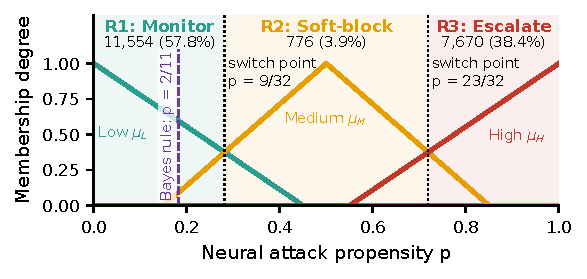
\includegraphics{figures/fig1_decision_bands.pdf}
\caption{Fuzzy mapping from attack propensity to action (seed-42 test set). Rules $R_1$--$R_3$ switch action at $p=9/32$ and $23/32$ (dotted); dashed: Bayes soft-block threshold $p=2/11$. The Soft-block band (776 alerts, 3.9\%) yields the entire cost gain over the 0.5 threshold.}
\label{fig:bands}
\end{figure}

\textit{Cost model and decision metrics.} Actions are scored with the relative cost matrix
\begin{equation}
\begin{aligned}
C(\text{Monitor},y)&=C_{FN}\,y, & C(\text{Soft-block},y)&=1+(1-y),\\
C(\text{Escalate},y)&=3+3(1-y), & C_{FN}&=10.
\end{aligned}
\label{eq:cost}
\end{equation}
Policies are compared by the mean triage cost $\bar C=(1/N)\sum_i C(a_i,y_i)$, the attack coverage $\sum_i \mathbf{1}[a_i\neq\text{Monitor}]\,y_i/\sum_i y_i$ and the number of unnecessary escalations (UE), that is, benign alerts sent to an analyst. As a reference, we report the plug-in Bayes cost rule
\begin{equation}
a_i^{B}=\arg\min_{a}\;\big[(1-p_i)\,C(a,0)+p_i\,C(a,1)\big].
\label{eq:bayes}
\end{equation}
which treats $p_i$ as calibrated, although deep-model scores do not guarantee calibration~\cite{abdar2021}. Because soft-blocking is cheaper than escalation for both classes, this rule never escalates and soft-blocks every alert with $p_i>2/11$.

%% ---------------------------------------------------------------------------
\section{Experimental design}
\label{sec:design}
\textit{Data.} We used the NSL-KDD benchmark~\cite{tavallaee2009}. 40,000 training records were sampled and split, with stratification, into 34,000 training and 6,000 validation records, and the scaler and encoder were fitted on the training split only. The test set was capped at 20,000 records (attack rate 0.568) and contains attack types absent from training.

\textit{Baselines.} The detectors were class-balanced logistic regression, gradient boosting (GB)~\cite{friedman2001} with scikit-learn defaults, and the MLP alone. The proposed policy uses the MLP propensity, so any benefit comes from better decisions rather than better scores. Three decision baselines acted on the same scores: a 0.5 threshold that escalates alerts above it and monitors the rest, the same threshold tuned on validation data to minimise cost (threshold moving~\cite{zhou2006}), and escalation of the 20\% highest-scored alerts, which mimics a fixed analyst capacity.

\textit{Statistics.} On the seed-42 test set, percentile 95\% confidence intervals (CIs) come from 2,000 paired bootstrap resamples~\cite{efron1994}, and per-alert cost differences were tested with the two-sided Wilcoxon signed-rank test~\cite{wilcoxon1945}, which treats alerts as independent. The pipeline was repeated for seeds 42--51, with seed-level costs compared by a paired Wilcoxon test. Sensitivity sweeps varied $C_{FN}$ and the Medium half-width.

%% ---------------------------------------------------------------------------
\section{Results and discussion}
\label{sec:results}
\begin{table}[!t]
\centering
\caption{Main results on the seed-42 test set ($N=20{,}000$ alerts).}
\label{tab:main}
\setlength{\tabcolsep}{4pt}
\resizebox{\linewidth}{!}{%
\begin{tabular}{@{}llcccccc@{}}
\toprule
\multicolumn{8}{@{}l}{\textit{Panel A. Detector quality (threshold 0.5 for accuracy and F1)}}\\
Detector & & Accuracy & F1 & ROC-AUC & PR-AUC & & ROC-AUC, 10 seeds \\
\midrule
Logistic regression & & 0.752 & 0.740 & 0.818 & 0.879 & & $0.812\pm0.008$ \\
Gradient boosting & & \textbf{0.786} & \textbf{0.774} & \textbf{0.947} & \textbf{0.951} & & $\mathbf{0.936\pm0.010}$ \\
MLP (input to proposed policy) & & 0.773 & 0.766 & 0.908 & 0.923 & & $0.900\pm0.007$ \\
\midrule
\multicolumn{8}{@{}l}{\textit{Panel B. Decision policies on identical MLP scores}}\\
Policy & Scores & $\bar C$ & Coverage & UE & $\Delta\bar C$ & $p$ & $\bar C$, 10 seeds \\
\midrule
Threshold 0.5 & MLP & \makecell{3.264\\{\scriptsize [3.210, 3.316]}} & \makecell{0.655\\{\scriptsize [0.646, 0.664]}} & 623 & \makecell{$+0.196$\\{\scriptsize [0.180, 0.213]}} & $7.3{\times}10^{-124}$ & $3.246\pm0.076$ \\
Top-20\% escalation & MLP & \makecell{4.309\\{\scriptsize [4.246, 4.372]}} & \makecell{0.348\\{\scriptsize [0.339, 0.357]}} & \textbf{47} & \makecell{$+1.242$\\{\scriptsize [1.196, 1.285]}} & $<10^{-300}$ & $4.318\pm0.009$ \\
\textbf{Fuzzy rule policy (proposed)} & MLP & \makecell{\textbf{3.068}\\{\scriptsize [3.016, 3.118]}} & \makecell{\textbf{0.686}\\{\scriptsize [0.677, 0.694]}} & 603 & -- & -- & $\mathbf{3.088\pm0.081}$ \\
\bottomrule
\end{tabular}}
\par\smallskip
\parbox{\linewidth}{\scriptsize\raggedright Brackets: paired bootstrap 95\% CIs. $\Delta\bar C$: cost difference from the proposed policy. $p$: two-sided Wilcoxon signed-rank test on per-alert costs. 10 seeds: mean $\pm$ SD over seeds 42--51. Bold: best in each panel. PR-AUC: area under the precision--recall curve. $\bar C$: mean triage cost, Eq.~(\ref{eq:cost}). UE: unnecessary escalations. Ablation and reference policies, with CIs: Supplementary Material (\texttt{table2\_decision.csv}).}
\end{table}

\textit{Prediction versus decision.} Gradient boosting is the best detector on every metric and beats the MLP in ROC-AUC in all ten seeds (Table~\ref{tab:main}, Panel A), so we make no claim about detection. On identical MLP scores, however, the rule base lowers the mean triage cost by 0.196 per alert relative to the 0.5 threshold and by 1.242 relative to top-20\% escalation, and it raises coverage by 0.031 over the threshold (95\% CI [0.028, 0.034]; Panel B). The two policies differ only on the 776 Medium-band alerts, which are contained instead of monitored or escalated, saving about 3,900 cost units per 20,000 alerts and sending 387 fewer alerts to analysts.

\begin{figure}[!tb]
\centering
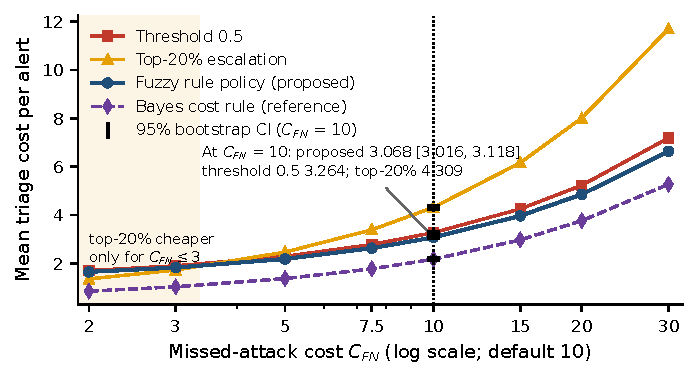
\includegraphics{figures/fig2_cost_sensitivity.pdf}
\caption{Mean triage cost against the missed-attack cost $C_{FN}$ (seed 42, log axis). Top-20\% escalation is cheaper than the fuzzy rule policy only for $C_{FN}\le3$ (shaded). Error bars: paired bootstrap 95\% CIs at the default $C_{FN}=10$ (dotted); dashed: Bayes reference.}
\label{fig:sens}
\end{figure}

\textit{Robustness.} The rule base is cheaper than both crisp rules in every seed (Wilcoxon $p=0.002$ for both; means in Table~\ref{tab:main}), and its coverage exceeds that of the threshold in every seed. Its advantage over the threshold grows from 0.055 at $C_{FN}=2$ to 0.549 at $C_{FN}=30$ (Fig.~\ref{fig:sens}), whereas top-20\% escalation is cheaper only when $C_{FN}\le3$ (1.347 against 1.640 at $C_{FN}=2$). Widening the Medium half-width from 0.25 to 0.45 enlarges the Soft-block band from 646 to 900 alerts and lowers the cost from 3.101 to 3.034, and every width beats both crisp rules.

\textit{Sources and limits of the gain.} Crisp bands with cut-points at $p=9/32$ and $23/32$ reproduce every action of the rule base (ablations in the Supplementary Material), so the gain comes from the intermediate containment band, while fuzziness adds a graded explanation of each decision. The rule base is not cost-optimal: the Bayes cost rule soft-blocks 8,631 alerts (43\% of traffic) and is 0.903 cheaper per alert. Validation tuning moves the threshold only to $t=0.53$ (cost 3.278), and only an oracle threshold of 0.10 or lower, chosen on the test set, would beat the rule base (2.929 at $t=0.01$). On GB scores, the same rules cost 3.004, lower than on MLP scores ($p=0.017$), and cut unnecessary escalations from 603 to 222.

\textit{Implications for SOC decision-makers.} Detectors should be judged by the decisions they enable: the action rule alone changed the cost by up to 1.242 per alert. Unlike a deferral band~\cite{jalalvand2027}, Soft-block acts without an analyst, so false containment must be priced before it is automated. The band boundaries give managers a workload lever without retraining, useful when false positives dominate alert streams~\cite{albasheer2022}, and logged firing strengths give each action an audit trail that post hoc attributions lack~\cite{wang2020xai,alabbadi2025}.

\textit{Limitations.} The study has four limitations. First, fixed bands respond to the distribution of the scores, not only to their ranking. Seed 48, the weakest replicate (cost 3.282, coverage 0.626), has a typical ROC-AUC of 0.900 but the lowest accuracy at the 0.5 threshold (0.757). Second, NSL-KDD is a laboratory benchmark released in 2009~\cite{tavallaee2009} that predates modern enterprise and cloud traffic, and it was subsampled under a single protocol. Third, the cost matrix is illustrative rather than elicited from a real SOC, and coverage counts containment as covering an attack. Fourth, there was no deployment, drift analysis or user study.

\section{Conclusion}
\label{sec:concl}
A fuzzy--neural rule base can serve as a knowledge-based decision layer for alert triage: on NSL-KDD, it achieved lower cost and higher coverage than crisp threshold and capacity rules across seeds, cost ratios and band widths, through its intermediate containment band. Future work will elicit real SOC costs, test the layer in live operation and bound automatic-action errors by conformal classification with a reject option~\cite{szabadvary2025}.

%% ---------------------------------------------------------------------------
\section*{Data availability}
The code, results (with the ablations in \texttt{table2\_decision.csv}) and figure scripts are in the Supplementary Material and at \url{https://github.com/nithin427/fuzzy-neural-cyber-triage}. NSL-KDD is available from the Canadian Institute for Cybersecurity at \url{https://www.unb.ca/cic/datasets/nsl.html}~\cite{tavallaee2009}.

\section*{Declaration of competing interest}
The author declares no known competing financial interests or personal relationships that could have appeared to influence the work reported in this paper.

\section*{Declaration of generative AI and AI-assisted technologies in the manuscript preparation process}
During the preparation of this work the author used Grok Bot, an AI-assisted writing and coding tool, to help with language editing, code refactoring, reference checking and formatting. After using this tool, the author reviewed and edited the content as needed and takes full responsibility for the content of the published article.

\section*{Funding}
This research did not receive any specific grant from funding agencies in the public, commercial, or not-for-profit sectors.

\section*{CRediT authorship contribution statement}
\textbf{Sai Nithin Erigineni:} Conceptualization, Methodology, Software, Validation, Formal analysis, Investigation, Data curation, Visualization, Writing -- original draft, Writing -- review \& editing.

\renewcommand{\bibfont}{\fontsize{8.5}{9.5}\selectfont}\setlength{\bibsep}{0pt plus 0.5pt}
\bibliographystyle{elsarticle-num}
\bibliography{refs}
\end{document}
